% Created by tikzDevice version 0.12.3.1 on 2023-02-21 12:15:55
% !TEX encoding = UTF-8 Unicode
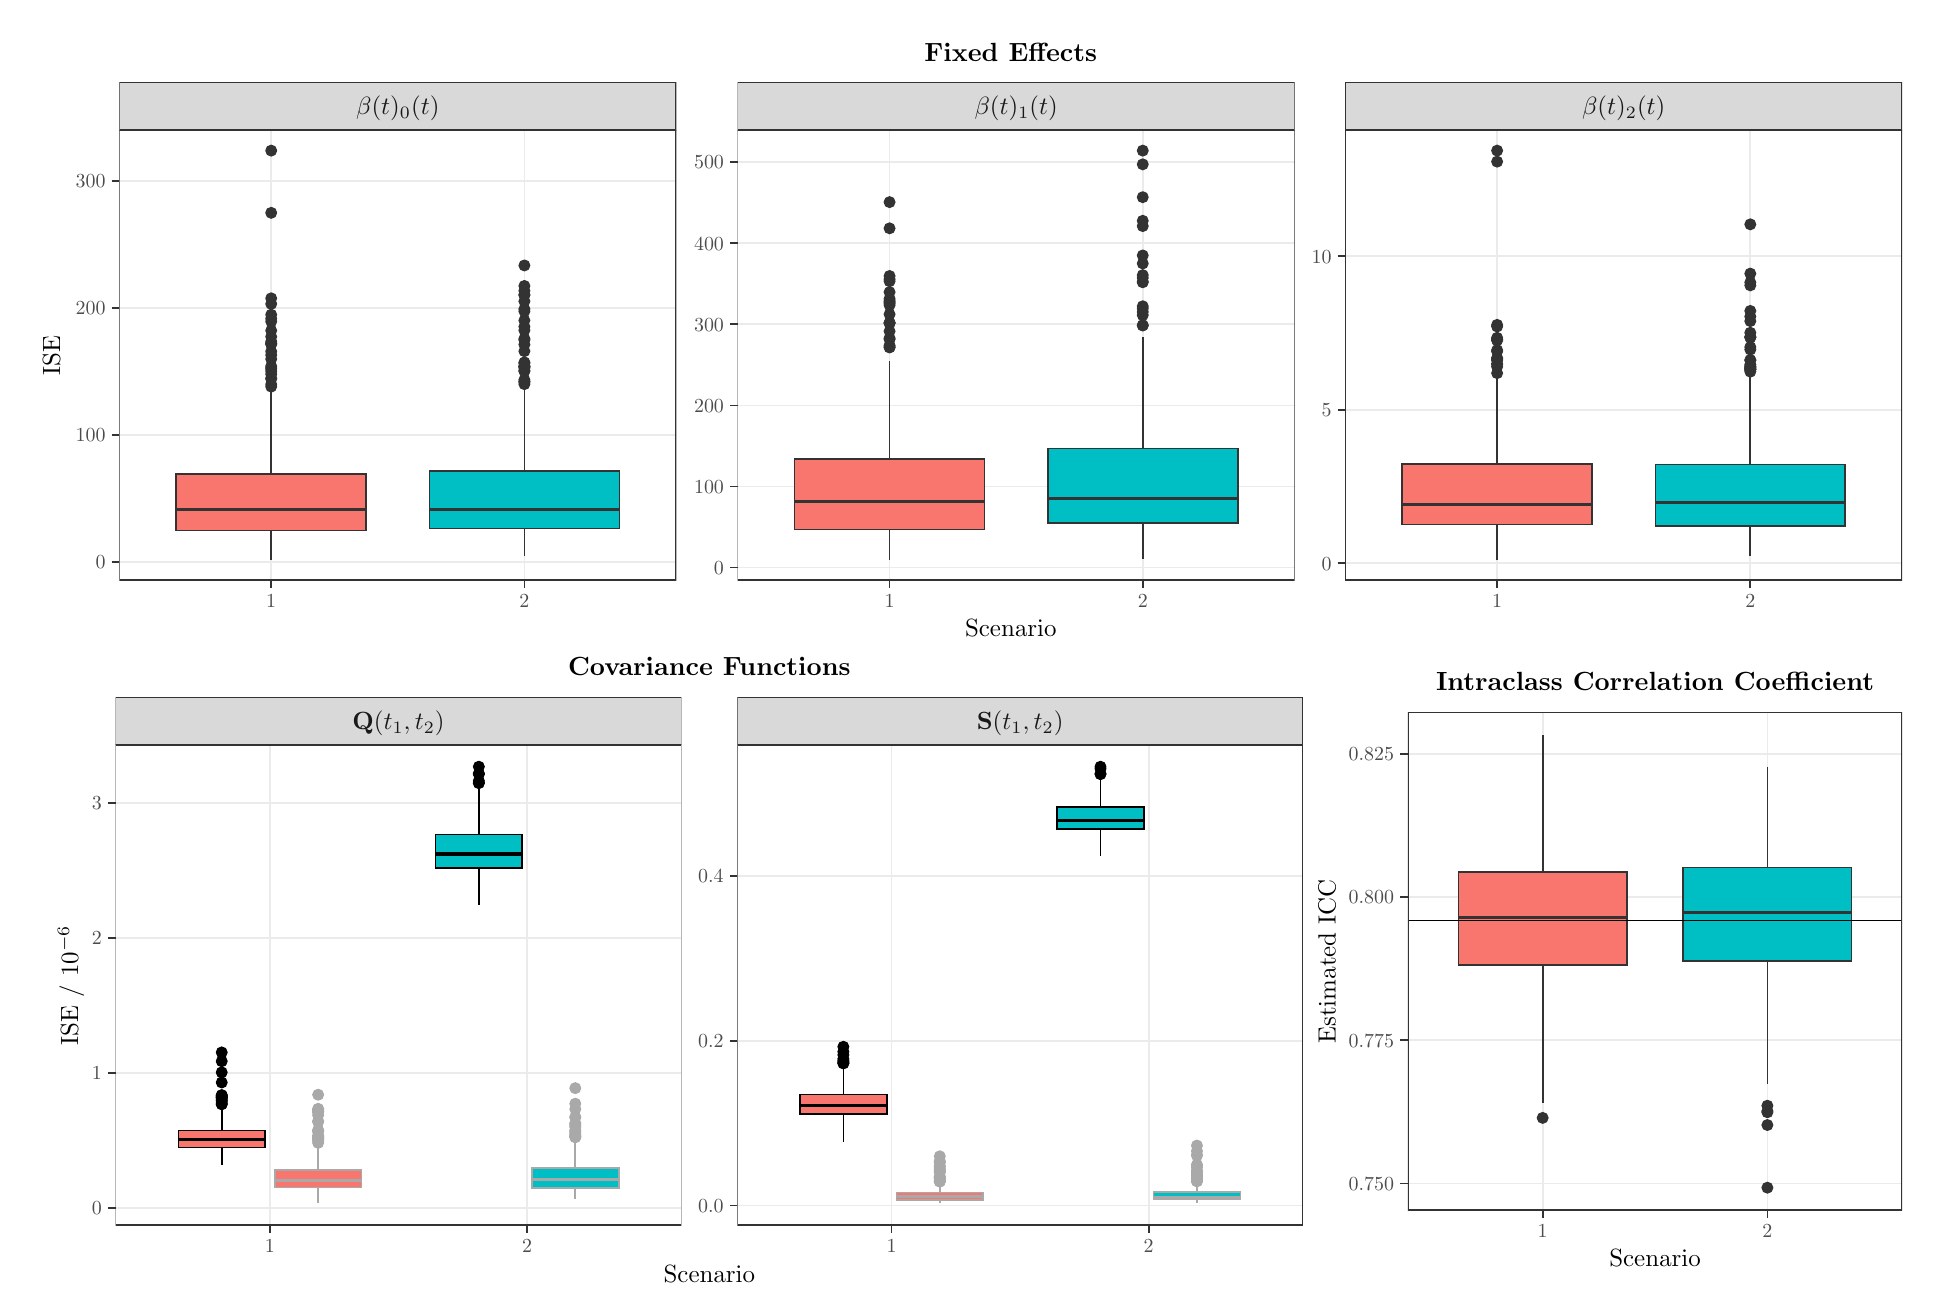
\begin{tikzpicture}[x=1pt,y=1pt]
\definecolor{fillColor}{RGB}{255,255,255}
\path[use as bounding box,fill=fillColor,fill opacity=0.00] (0,0) rectangle (682.86,455.24);
\begin{scope}
\path[clip] (  0.00,227.62) rectangle (682.86,455.24);
\definecolor{drawColor}{RGB}{255,255,255}
\definecolor{fillColor}{RGB}{255,255,255}

\path[draw=drawColor,line width= 0.6pt,line join=round,line cap=round,fill=fillColor] (  0.00,227.62) rectangle (682.86,455.24);
\end{scope}
\begin{scope}
\path[clip] ( 33.11,255.60) rectangle (234.38,418.21);
\definecolor{fillColor}{RGB}{255,255,255}

\path[fill=fillColor] ( 33.11,255.60) rectangle (234.38,418.21);
\definecolor{drawColor}{gray}{0.92}

\path[draw=drawColor,line width= 0.6pt,line join=round] ( 33.11,262.26) --
	(234.38,262.26);

\path[draw=drawColor,line width= 0.6pt,line join=round] ( 33.11,308.12) --
	(234.38,308.12);

\path[draw=drawColor,line width= 0.6pt,line join=round] ( 33.11,353.98) --
	(234.38,353.98);

\path[draw=drawColor,line width= 0.6pt,line join=round] ( 33.11,399.85) --
	(234.38,399.85);

\path[draw=drawColor,line width= 0.6pt,line join=round] ( 88.00,255.60) --
	( 88.00,418.21);

\path[draw=drawColor,line width= 0.6pt,line join=round] (179.49,255.60) --
	(179.49,418.21);
\definecolor{drawColor}{gray}{0.20}
\definecolor{fillColor}{gray}{0.20}

\path[draw=drawColor,line width= 0.4pt,line join=round,line cap=round,fill=fillColor] ( 88.00,341.16) circle (  1.96);

\path[draw=drawColor,line width= 0.4pt,line join=round,line cap=round,fill=fillColor] ( 88.00,351.52) circle (  1.96);

\path[draw=drawColor,line width= 0.4pt,line join=round,line cap=round,fill=fillColor] ( 88.00,328.55) circle (  1.96);

\path[draw=drawColor,line width= 0.4pt,line join=round,line cap=round,fill=fillColor] ( 88.00,357.44) circle (  1.96);

\path[draw=drawColor,line width= 0.4pt,line join=round,line cap=round,fill=fillColor] ( 88.00,332.32) circle (  1.96);

\path[draw=drawColor,line width= 0.4pt,line join=round,line cap=round,fill=fillColor] ( 88.00,349.05) circle (  1.96);

\path[draw=drawColor,line width= 0.4pt,line join=round,line cap=round,fill=fillColor] ( 88.00,345.80) circle (  1.96);

\path[draw=drawColor,line width= 0.4pt,line join=round,line cap=round,fill=fillColor] ( 88.00,340.93) circle (  1.96);

\path[draw=drawColor,line width= 0.4pt,line join=round,line cap=round,fill=fillColor] ( 88.00,338.26) circle (  1.96);

\path[draw=drawColor,line width= 0.4pt,line join=round,line cap=round,fill=fillColor] ( 88.00,336.95) circle (  1.96);

\path[draw=drawColor,line width= 0.4pt,line join=round,line cap=round,fill=fillColor] ( 88.00,328.36) circle (  1.96);

\path[draw=drawColor,line width= 0.4pt,line join=round,line cap=round,fill=fillColor] ( 88.00,325.53) circle (  1.96);

\path[draw=drawColor,line width= 0.4pt,line join=round,line cap=round,fill=fillColor] ( 88.00,350.13) circle (  1.96);

\path[draw=drawColor,line width= 0.4pt,line join=round,line cap=round,fill=fillColor] ( 88.00,410.81) circle (  1.96);

\path[draw=drawColor,line width= 0.4pt,line join=round,line cap=round,fill=fillColor] ( 88.00,330.01) circle (  1.96);

\path[draw=drawColor,line width= 0.4pt,line join=round,line cap=round,fill=fillColor] ( 88.00,335.50) circle (  1.96);

\path[draw=drawColor,line width= 0.4pt,line join=round,line cap=round,fill=fillColor] ( 88.00,331.87) circle (  1.96);

\path[draw=drawColor,line width= 0.4pt,line join=round,line cap=round,fill=fillColor] ( 88.00,343.57) circle (  1.96);

\path[draw=drawColor,line width= 0.4pt,line join=round,line cap=round,fill=fillColor] ( 88.00,331.05) circle (  1.96);

\path[draw=drawColor,line width= 0.4pt,line join=round,line cap=round,fill=fillColor] ( 88.00,388.33) circle (  1.96);

\path[draw=drawColor,line width= 0.4pt,line join=round,line cap=round,fill=fillColor] ( 88.00,332.92) circle (  1.96);

\path[draw=drawColor,line width= 0.4pt,line join=round,line cap=round,fill=fillColor] ( 88.00,340.93) circle (  1.96);

\path[draw=drawColor,line width= 0.4pt,line join=round,line cap=round,fill=fillColor] ( 88.00,326.35) circle (  1.96);

\path[draw=drawColor,line width= 0.4pt,line join=round,line cap=round,fill=fillColor] ( 88.00,341.83) circle (  1.96);

\path[draw=drawColor,line width= 0.4pt,line join=round,line cap=round,fill=fillColor] ( 88.00,355.42) circle (  1.96);

\path[draw=drawColor,line width= 0.6pt,line join=round] ( 88.00,294.03) -- ( 88.00,324.57);

\path[draw=drawColor,line width= 0.6pt,line join=round] ( 88.00,273.50) -- ( 88.00,262.99);
\definecolor{fillColor}{RGB}{248,118,109}

\path[draw=drawColor,line width= 0.6pt,fill=fillColor] ( 53.69,294.03) --
	( 53.69,273.50) --
	(122.31,273.50) --
	(122.31,294.03) --
	( 53.69,294.03) --
	cycle;

\path[draw=drawColor,line width= 1.1pt] ( 53.69,281.27) -- (122.31,281.27);
\definecolor{fillColor}{gray}{0.20}

\path[draw=drawColor,line width= 0.4pt,line join=round,line cap=round,fill=fillColor] (179.49,353.58) circle (  1.96);

\path[draw=drawColor,line width= 0.4pt,line join=round,line cap=round,fill=fillColor] (179.49,328.00) circle (  1.96);

\path[draw=drawColor,line width= 0.4pt,line join=round,line cap=round,fill=fillColor] (179.49,332.66) circle (  1.96);

\path[draw=drawColor,line width= 0.4pt,line join=round,line cap=round,fill=fillColor] (179.49,331.07) circle (  1.96);

\path[draw=drawColor,line width= 0.4pt,line join=round,line cap=round,fill=fillColor] (179.49,334.29) circle (  1.96);

\path[draw=drawColor,line width= 0.4pt,line join=round,line cap=round,fill=fillColor] (179.49,358.57) circle (  1.96);

\path[draw=drawColor,line width= 0.4pt,line join=round,line cap=round,fill=fillColor] (179.49,340.72) circle (  1.96);

\path[draw=drawColor,line width= 0.4pt,line join=round,line cap=round,fill=fillColor] (179.49,331.36) circle (  1.96);

\path[draw=drawColor,line width= 0.4pt,line join=round,line cap=round,fill=fillColor] (179.49,360.15) circle (  1.96);

\path[draw=drawColor,line width= 0.4pt,line join=round,line cap=round,fill=fillColor] (179.49,332.30) circle (  1.96);

\path[draw=drawColor,line width= 0.4pt,line join=round,line cap=round,fill=fillColor] (179.49,333.99) circle (  1.96);

\path[draw=drawColor,line width= 0.4pt,line join=round,line cap=round,fill=fillColor] (179.49,327.23) circle (  1.96);

\path[draw=drawColor,line width= 0.4pt,line join=round,line cap=round,fill=fillColor] (179.49,349.46) circle (  1.96);

\path[draw=drawColor,line width= 0.4pt,line join=round,line cap=round,fill=fillColor] (179.49,358.74) circle (  1.96);

\path[draw=drawColor,line width= 0.4pt,line join=round,line cap=round,fill=fillColor] (179.49,352.75) circle (  1.96);

\path[draw=drawColor,line width= 0.4pt,line join=round,line cap=round,fill=fillColor] (179.49,342.86) circle (  1.96);

\path[draw=drawColor,line width= 0.4pt,line join=round,line cap=round,fill=fillColor] (179.49,356.37) circle (  1.96);

\path[draw=drawColor,line width= 0.4pt,line join=round,line cap=round,fill=fillColor] (179.49,338.34) circle (  1.96);

\path[draw=drawColor,line width= 0.4pt,line join=round,line cap=round,fill=fillColor] (179.49,327.32) circle (  1.96);

\path[draw=drawColor,line width= 0.4pt,line join=round,line cap=round,fill=fillColor] (179.49,332.80) circle (  1.96);

\path[draw=drawColor,line width= 0.4pt,line join=round,line cap=round,fill=fillColor] (179.49,326.43) circle (  1.96);

\path[draw=drawColor,line width= 0.4pt,line join=round,line cap=round,fill=fillColor] (179.49,333.04) circle (  1.96);

\path[draw=drawColor,line width= 0.4pt,line join=round,line cap=round,fill=fillColor] (179.49,361.91) circle (  1.96);

\path[draw=drawColor,line width= 0.4pt,line join=round,line cap=round,fill=fillColor] (179.49,369.32) circle (  1.96);

\path[draw=drawColor,line width= 0.4pt,line join=round,line cap=round,fill=fillColor] (179.49,345.88) circle (  1.96);

\path[draw=drawColor,line width= 0.4pt,line join=round,line cap=round,fill=fillColor] (179.49,347.18) circle (  1.96);

\path[draw=drawColor,line width= 0.4pt,line join=round,line cap=round,fill=fillColor] (179.49,342.37) circle (  1.96);

\path[draw=drawColor,line width= 0.6pt,line join=round] (179.49,295.01) -- (179.49,324.23);

\path[draw=drawColor,line width= 0.6pt,line join=round] (179.49,274.28) -- (179.49,264.41);
\definecolor{fillColor}{RGB}{0,191,196}

\path[draw=drawColor,line width= 0.6pt,fill=fillColor] (145.18,295.01) --
	(145.18,274.28) --
	(213.80,274.28) --
	(213.80,295.01) --
	(145.18,295.01) --
	cycle;

\path[draw=drawColor,line width= 1.1pt] (145.18,281.06) -- (213.80,281.06);

\path[draw=drawColor,line width= 0.6pt,line join=round,line cap=round] ( 33.11,255.60) rectangle (234.38,418.21);
\end{scope}
\begin{scope}
\path[clip] (256.55,255.60) rectangle (457.83,418.21);
\definecolor{fillColor}{RGB}{255,255,255}

\path[fill=fillColor] (256.55,255.60) rectangle (457.83,418.21);
\definecolor{drawColor}{gray}{0.92}

\path[draw=drawColor,line width= 0.6pt,line join=round] (256.55,260.15) --
	(457.83,260.15);

\path[draw=drawColor,line width= 0.6pt,line join=round] (256.55,289.46) --
	(457.83,289.46);

\path[draw=drawColor,line width= 0.6pt,line join=round] (256.55,318.76) --
	(457.83,318.76);

\path[draw=drawColor,line width= 0.6pt,line join=round] (256.55,348.07) --
	(457.83,348.07);

\path[draw=drawColor,line width= 0.6pt,line join=round] (256.55,377.37) --
	(457.83,377.37);

\path[draw=drawColor,line width= 0.6pt,line join=round] (256.55,406.68) --
	(457.83,406.68);

\path[draw=drawColor,line width= 0.6pt,line join=round] (311.44,255.60) --
	(311.44,418.21);

\path[draw=drawColor,line width= 0.6pt,line join=round] (402.93,255.60) --
	(402.93,418.21);
\definecolor{drawColor}{gray}{0.20}
\definecolor{fillColor}{gray}{0.20}

\path[draw=drawColor,line width= 0.4pt,line join=round,line cap=round,fill=fillColor] (311.44,339.83) circle (  1.96);

\path[draw=drawColor,line width= 0.4pt,line join=round,line cap=round,fill=fillColor] (311.44,364.39) circle (  1.96);

\path[draw=drawColor,line width= 0.4pt,line join=round,line cap=round,fill=fillColor] (311.44,382.73) circle (  1.96);

\path[draw=drawColor,line width= 0.4pt,line join=round,line cap=round,fill=fillColor] (311.44,392.20) circle (  1.96);

\path[draw=drawColor,line width= 0.4pt,line join=round,line cap=round,fill=fillColor] (311.44,356.54) circle (  1.96);

\path[draw=drawColor,line width= 0.4pt,line join=round,line cap=round,fill=fillColor] (311.44,342.62) circle (  1.96);

\path[draw=drawColor,line width= 0.4pt,line join=round,line cap=round,fill=fillColor] (311.44,365.51) circle (  1.96);

\path[draw=drawColor,line width= 0.4pt,line join=round,line cap=round,fill=fillColor] (311.44,343.05) circle (  1.96);

\path[draw=drawColor,line width= 0.4pt,line join=round,line cap=round,fill=fillColor] (311.44,348.60) circle (  1.96);

\path[draw=drawColor,line width= 0.4pt,line join=round,line cap=round,fill=fillColor] (311.44,359.69) circle (  1.96);

\path[draw=drawColor,line width= 0.4pt,line join=round,line cap=round,fill=fillColor] (311.44,348.51) circle (  1.96);

\path[draw=drawColor,line width= 0.4pt,line join=round,line cap=round,fill=fillColor] (311.44,354.95) circle (  1.96);

\path[draw=drawColor,line width= 0.4pt,line join=round,line cap=round,fill=fillColor] (311.44,340.44) circle (  1.96);

\path[draw=drawColor,line width= 0.4pt,line join=round,line cap=round,fill=fillColor] (311.44,345.55) circle (  1.96);

\path[draw=drawColor,line width= 0.4pt,line join=round,line cap=round,fill=fillColor] (311.44,355.63) circle (  1.96);

\path[draw=drawColor,line width= 0.4pt,line join=round,line cap=round,fill=fillColor] (311.44,348.51) circle (  1.96);

\path[draw=drawColor,line width= 0.4pt,line join=round,line cap=round,fill=fillColor] (311.44,356.06) circle (  1.96);

\path[draw=drawColor,line width= 0.4pt,line join=round,line cap=round,fill=fillColor] (311.44,363.61) circle (  1.96);

\path[draw=drawColor,line width= 0.4pt,line join=round,line cap=round,fill=fillColor] (311.44,357.29) circle (  1.96);

\path[draw=drawColor,line width= 0.4pt,line join=round,line cap=round,fill=fillColor] (311.44,351.68) circle (  1.96);

\path[draw=drawColor,line width= 0.4pt,line join=round,line cap=round,fill=fillColor] (311.44,339.68) circle (  1.96);

\path[draw=drawColor,line width= 0.6pt,line join=round] (311.44,299.46) -- (311.44,334.71);

\path[draw=drawColor,line width= 0.6pt,line join=round] (311.44,273.93) -- (311.44,262.99);
\definecolor{fillColor}{RGB}{248,118,109}

\path[draw=drawColor,line width= 0.6pt,fill=fillColor] (277.14,299.46) --
	(277.14,273.93) --
	(345.75,273.93) --
	(345.75,299.46) --
	(277.14,299.46) --
	cycle;

\path[draw=drawColor,line width= 1.1pt] (277.14,283.97) -- (345.75,283.97);
\definecolor{fillColor}{gray}{0.20}

\path[draw=drawColor,line width= 0.4pt,line join=round,line cap=round,fill=fillColor] (402.93,353.75) circle (  1.96);

\path[draw=drawColor,line width= 0.4pt,line join=round,line cap=round,fill=fillColor] (402.93,370.03) circle (  1.96);

\path[draw=drawColor,line width= 0.4pt,line join=round,line cap=round,fill=fillColor] (402.93,365.82) circle (  1.96);

\path[draw=drawColor,line width= 0.4pt,line join=round,line cap=round,fill=fillColor] (402.93,352.53) circle (  1.96);

\path[draw=drawColor,line width= 0.4pt,line join=round,line cap=round,fill=fillColor] (402.93,354.57) circle (  1.96);

\path[draw=drawColor,line width= 0.4pt,line join=round,line cap=round,fill=fillColor] (402.93,363.23) circle (  1.96);

\path[draw=drawColor,line width= 0.4pt,line join=round,line cap=round,fill=fillColor] (402.93,383.54) circle (  1.96);

\path[draw=drawColor,line width= 0.4pt,line join=round,line cap=round,fill=fillColor] (402.93,363.46) circle (  1.96);

\path[draw=drawColor,line width= 0.4pt,line join=round,line cap=round,fill=fillColor] (402.93,351.36) circle (  1.96);

\path[draw=drawColor,line width= 0.4pt,line join=round,line cap=round,fill=fillColor] (402.93,347.62) circle (  1.96);

\path[draw=drawColor,line width= 0.4pt,line join=round,line cap=round,fill=fillColor] (402.93,364.84) circle (  1.96);

\path[draw=drawColor,line width= 0.4pt,line join=round,line cap=round,fill=fillColor] (402.93,393.98) circle (  1.96);

\path[draw=drawColor,line width= 0.4pt,line join=round,line cap=round,fill=fillColor] (402.93,372.93) circle (  1.96);

\path[draw=drawColor,line width= 0.4pt,line join=round,line cap=round,fill=fillColor] (402.93,405.85) circle (  1.96);

\path[draw=drawColor,line width= 0.4pt,line join=round,line cap=round,fill=fillColor] (402.93,410.81) circle (  1.96);

\path[draw=drawColor,line width= 0.4pt,line join=round,line cap=round,fill=fillColor] (402.93,385.45) circle (  1.96);

\path[draw=drawColor,line width= 0.4pt,line join=round,line cap=round,fill=fillColor] (402.93,347.71) circle (  1.96);

\path[draw=drawColor,line width= 0.6pt,line join=round] (402.93,303.18) -- (402.93,343.55);

\path[draw=drawColor,line width= 0.6pt,line join=round] (402.93,276.20) -- (402.93,263.30);
\definecolor{fillColor}{RGB}{0,191,196}

\path[draw=drawColor,line width= 0.6pt,fill=fillColor] (368.62,303.18) --
	(368.62,276.20) --
	(437.24,276.20) --
	(437.24,303.18) --
	(368.62,303.18) --
	cycle;

\path[draw=drawColor,line width= 1.1pt] (368.62,285.13) -- (437.24,285.13);

\path[draw=drawColor,line width= 0.6pt,line join=round,line cap=round] (256.55,255.60) rectangle (457.83,418.21);
\end{scope}
\begin{scope}
\path[clip] (476.09,255.60) rectangle (677.36,418.21);
\definecolor{fillColor}{RGB}{255,255,255}

\path[fill=fillColor] (476.09,255.60) rectangle (677.36,418.21);
\definecolor{drawColor}{gray}{0.92}

\path[draw=drawColor,line width= 0.6pt,line join=round] (476.09,261.74) --
	(677.36,261.74);

\path[draw=drawColor,line width= 0.6pt,line join=round] (476.09,317.18) --
	(677.36,317.18);

\path[draw=drawColor,line width= 0.6pt,line join=round] (476.09,372.62) --
	(677.36,372.62);

\path[draw=drawColor,line width= 0.6pt,line join=round] (530.98,255.60) --
	(530.98,418.21);

\path[draw=drawColor,line width= 0.6pt,line join=round] (622.47,255.60) --
	(622.47,418.21);
\definecolor{drawColor}{gray}{0.20}
\definecolor{fillColor}{gray}{0.20}

\path[draw=drawColor,line width= 0.4pt,line join=round,line cap=round,fill=fillColor] (530.98,347.85) circle (  1.96);

\path[draw=drawColor,line width= 0.4pt,line join=round,line cap=round,fill=fillColor] (530.98,338.72) circle (  1.96);

\path[draw=drawColor,line width= 0.4pt,line join=round,line cap=round,fill=fillColor] (530.98,332.71) circle (  1.96);

\path[draw=drawColor,line width= 0.4pt,line join=round,line cap=round,fill=fillColor] (530.98,330.40) circle (  1.96);

\path[draw=drawColor,line width= 0.4pt,line join=round,line cap=round,fill=fillColor] (530.98,347.26) circle (  1.96);

\path[draw=drawColor,line width= 0.4pt,line join=round,line cap=round,fill=fillColor] (530.98,343.17) circle (  1.96);

\path[draw=drawColor,line width= 0.4pt,line join=round,line cap=round,fill=fillColor] (530.98,410.81) circle (  1.96);

\path[draw=drawColor,line width= 0.4pt,line join=round,line cap=round,fill=fillColor] (530.98,335.73) circle (  1.96);

\path[draw=drawColor,line width= 0.4pt,line join=round,line cap=round,fill=fillColor] (530.98,335.85) circle (  1.96);

\path[draw=drawColor,line width= 0.4pt,line join=round,line cap=round,fill=fillColor] (530.98,406.83) circle (  1.96);

\path[draw=drawColor,line width= 0.4pt,line join=round,line cap=round,fill=fillColor] (530.98,333.71) circle (  1.96);

\path[draw=drawColor,line width= 0.4pt,line join=round,line cap=round,fill=fillColor] (530.98,333.65) circle (  1.96);

\path[draw=drawColor,line width= 0.4pt,line join=round,line cap=round,fill=fillColor] (530.98,342.45) circle (  1.96);

\path[draw=drawColor,line width= 0.4pt,line join=round,line cap=round,fill=fillColor] (530.98,335.13) circle (  1.96);

\path[draw=drawColor,line width= 0.4pt,line join=round,line cap=round,fill=fillColor] (530.98,335.17) circle (  1.96);

\path[draw=drawColor,line width= 0.4pt,line join=round,line cap=round,fill=fillColor] (530.98,338.27) circle (  1.96);

\path[draw=drawColor,line width= 0.4pt,line join=round,line cap=round,fill=fillColor] (530.98,342.50) circle (  1.96);

\path[draw=drawColor,line width= 0.4pt,line join=round,line cap=round,fill=fillColor] (530.98,342.29) circle (  1.96);

\path[draw=drawColor,line width= 0.6pt,line join=round] (530.98,297.49) -- (530.98,329.17);

\path[draw=drawColor,line width= 0.6pt,line join=round] (530.98,275.69) -- (530.98,262.99);
\definecolor{fillColor}{RGB}{248,118,109}

\path[draw=drawColor,line width= 0.6pt,fill=fillColor] (496.67,297.49) --
	(496.67,275.69) --
	(565.29,275.69) --
	(565.29,297.49) --
	(496.67,297.49) --
	cycle;

\path[draw=drawColor,line width= 1.1pt] (496.67,282.79) -- (565.29,282.79);
\definecolor{fillColor}{gray}{0.20}

\path[draw=drawColor,line width= 0.4pt,line join=round,line cap=round,fill=fillColor] (622.47,343.37) circle (  1.96);

\path[draw=drawColor,line width= 0.4pt,line join=round,line cap=round,fill=fillColor] (622.47,338.91) circle (  1.96);

\path[draw=drawColor,line width= 0.4pt,line join=round,line cap=round,fill=fillColor] (622.47,345.00) circle (  1.96);

\path[draw=drawColor,line width= 0.4pt,line join=round,line cap=round,fill=fillColor] (622.47,331.66) circle (  1.96);

\path[draw=drawColor,line width= 0.4pt,line join=round,line cap=round,fill=fillColor] (622.47,335.01) circle (  1.96);

\path[draw=drawColor,line width= 0.4pt,line join=round,line cap=round,fill=fillColor] (622.47,366.37) circle (  1.96);

\path[draw=drawColor,line width= 0.4pt,line join=round,line cap=round,fill=fillColor] (622.47,331.70) circle (  1.96);

\path[draw=drawColor,line width= 0.4pt,line join=round,line cap=round,fill=fillColor] (622.47,332.42) circle (  1.96);

\path[draw=drawColor,line width= 0.4pt,line join=round,line cap=round,fill=fillColor] (622.47,362.12) circle (  1.96);

\path[draw=drawColor,line width= 0.4pt,line join=round,line cap=round,fill=fillColor] (622.47,343.33) circle (  1.96);

\path[draw=drawColor,line width= 0.4pt,line join=round,line cap=round,fill=fillColor] (622.47,384.17) circle (  1.96);

\path[draw=drawColor,line width= 0.4pt,line join=round,line cap=round,fill=fillColor] (622.47,349.21) circle (  1.96);

\path[draw=drawColor,line width= 0.4pt,line join=round,line cap=round,fill=fillColor] (622.47,343.51) circle (  1.96);

\path[draw=drawColor,line width= 0.4pt,line join=round,line cap=round,fill=fillColor] (622.47,335.16) circle (  1.96);

\path[draw=drawColor,line width= 0.4pt,line join=round,line cap=round,fill=fillColor] (622.47,332.88) circle (  1.96);

\path[draw=drawColor,line width= 0.4pt,line join=round,line cap=round,fill=fillColor] (622.47,339.84) circle (  1.96);

\path[draw=drawColor,line width= 0.4pt,line join=round,line cap=round,fill=fillColor] (622.47,363.19) circle (  1.96);

\path[draw=drawColor,line width= 0.4pt,line join=round,line cap=round,fill=fillColor] (622.47,332.64) circle (  1.96);

\path[draw=drawColor,line width= 0.4pt,line join=round,line cap=round,fill=fillColor] (622.47,332.03) circle (  1.96);

\path[draw=drawColor,line width= 0.4pt,line join=round,line cap=round,fill=fillColor] (622.47,330.94) circle (  1.96);

\path[draw=drawColor,line width= 0.4pt,line join=round,line cap=round,fill=fillColor] (622.47,350.86) circle (  1.96);

\path[draw=drawColor,line width= 0.4pt,line join=round,line cap=round,fill=fillColor] (622.47,352.88) circle (  1.96);

\path[draw=drawColor,line width= 0.4pt,line join=round,line cap=round,fill=fillColor] (622.47,331.78) circle (  1.96);

\path[draw=drawColor,line width= 0.4pt,line join=round,line cap=round,fill=fillColor] (622.47,333.50) circle (  1.96);

\path[draw=drawColor,line width= 0.6pt,line join=round] (622.47,297.40) -- (622.47,330.50);

\path[draw=drawColor,line width= 0.6pt,line join=round] (622.47,275.17) -- (622.47,264.48);
\definecolor{fillColor}{RGB}{0,191,196}

\path[draw=drawColor,line width= 0.6pt,fill=fillColor] (588.16,297.40) --
	(588.16,275.17) --
	(656.78,275.17) --
	(656.78,297.40) --
	(588.16,297.40) --
	cycle;

\path[draw=drawColor,line width= 1.1pt] (588.16,283.73) -- (656.78,283.73);

\path[draw=drawColor,line width= 0.6pt,line join=round,line cap=round] (476.09,255.60) rectangle (677.36,418.21);
\end{scope}
\begin{scope}
\path[clip] ( 33.11,418.21) rectangle (234.38,435.48);
\definecolor{drawColor}{gray}{0.20}
\definecolor{fillColor}{gray}{0.85}

\path[draw=drawColor,line width= 0.6pt,line join=round,line cap=round,fill=fillColor] ( 33.11,418.21) rectangle (234.38,435.48);
\definecolor{drawColor}{gray}{0.10}

\node[text=drawColor,anchor=base,inner sep=0pt, outer sep=0pt, scale=  0.90] at (133.74,423.74) {$\boldsymbol{\beta}(t)_0 (t)$};
\end{scope}
\begin{scope}
\path[clip] (256.55,418.21) rectangle (457.83,435.48);
\definecolor{drawColor}{gray}{0.20}
\definecolor{fillColor}{gray}{0.85}

\path[draw=drawColor,line width= 0.6pt,line join=round,line cap=round,fill=fillColor] (256.55,418.21) rectangle (457.83,435.48);
\definecolor{drawColor}{gray}{0.10}

\node[text=drawColor,anchor=base,inner sep=0pt, outer sep=0pt, scale=  0.90] at (357.19,423.74) {$\boldsymbol{\beta}(t)_1 (t)$};
\end{scope}
\begin{scope}
\path[clip] (476.09,418.21) rectangle (677.36,435.48);
\definecolor{drawColor}{gray}{0.20}
\definecolor{fillColor}{gray}{0.85}

\path[draw=drawColor,line width= 0.6pt,line join=round,line cap=round,fill=fillColor] (476.09,418.21) rectangle (677.36,435.48);
\definecolor{drawColor}{gray}{0.10}

\node[text=drawColor,anchor=base,inner sep=0pt, outer sep=0pt, scale=  0.90] at (576.73,423.74) {$\boldsymbol{\beta}(t)_2 (t)$};
\end{scope}
\begin{scope}
\path[clip] (  0.00,  0.00) rectangle (682.86,455.24);
\definecolor{drawColor}{gray}{0.20}

\path[draw=drawColor,line width= 0.6pt,line join=round] ( 88.00,252.85) --
	( 88.00,255.60);

\path[draw=drawColor,line width= 0.6pt,line join=round] (179.49,252.85) --
	(179.49,255.60);
\end{scope}
\begin{scope}
\path[clip] (  0.00,  0.00) rectangle (682.86,455.24);
\definecolor{drawColor}{gray}{0.30}

\node[text=drawColor,anchor=base,inner sep=0pt, outer sep=0pt, scale=  0.72] at ( 88.00,245.69) {1};

\node[text=drawColor,anchor=base,inner sep=0pt, outer sep=0pt, scale=  0.72] at (179.49,245.69) {2};
\end{scope}
\begin{scope}
\path[clip] (  0.00,  0.00) rectangle (682.86,455.24);
\definecolor{drawColor}{gray}{0.20}

\path[draw=drawColor,line width= 0.6pt,line join=round] (311.44,252.85) --
	(311.44,255.60);

\path[draw=drawColor,line width= 0.6pt,line join=round] (402.93,252.85) --
	(402.93,255.60);
\end{scope}
\begin{scope}
\path[clip] (  0.00,  0.00) rectangle (682.86,455.24);
\definecolor{drawColor}{gray}{0.30}

\node[text=drawColor,anchor=base,inner sep=0pt, outer sep=0pt, scale=  0.72] at (311.44,245.69) {1};

\node[text=drawColor,anchor=base,inner sep=0pt, outer sep=0pt, scale=  0.72] at (402.93,245.69) {2};
\end{scope}
\begin{scope}
\path[clip] (  0.00,  0.00) rectangle (682.86,455.24);
\definecolor{drawColor}{gray}{0.20}

\path[draw=drawColor,line width= 0.6pt,line join=round] (530.98,252.85) --
	(530.98,255.60);

\path[draw=drawColor,line width= 0.6pt,line join=round] (622.47,252.85) --
	(622.47,255.60);
\end{scope}
\begin{scope}
\path[clip] (  0.00,  0.00) rectangle (682.86,455.24);
\definecolor{drawColor}{gray}{0.30}

\node[text=drawColor,anchor=base,inner sep=0pt, outer sep=0pt, scale=  0.72] at (530.98,245.69) {1};

\node[text=drawColor,anchor=base,inner sep=0pt, outer sep=0pt, scale=  0.72] at (622.47,245.69) {2};
\end{scope}
\begin{scope}
\path[clip] (  0.00,  0.00) rectangle (682.86,455.24);
\definecolor{drawColor}{gray}{0.30}

\node[text=drawColor,anchor=base east,inner sep=0pt, outer sep=0pt, scale=  0.72] at (471.14,259.26) {0};

\node[text=drawColor,anchor=base east,inner sep=0pt, outer sep=0pt, scale=  0.72] at (471.14,314.70) {5};

\node[text=drawColor,anchor=base east,inner sep=0pt, outer sep=0pt, scale=  0.72] at (471.14,370.15) {10};
\end{scope}
\begin{scope}
\path[clip] (  0.00,  0.00) rectangle (682.86,455.24);
\definecolor{drawColor}{gray}{0.20}

\path[draw=drawColor,line width= 0.6pt,line join=round] (473.34,261.74) --
	(476.09,261.74);

\path[draw=drawColor,line width= 0.6pt,line join=round] (473.34,317.18) --
	(476.09,317.18);

\path[draw=drawColor,line width= 0.6pt,line join=round] (473.34,372.62) --
	(476.09,372.62);
\end{scope}
\begin{scope}
\path[clip] (  0.00,  0.00) rectangle (682.86,455.24);
\definecolor{drawColor}{gray}{0.30}

\node[text=drawColor,anchor=base east,inner sep=0pt, outer sep=0pt, scale=  0.72] at (251.60,257.67) {0};

\node[text=drawColor,anchor=base east,inner sep=0pt, outer sep=0pt, scale=  0.72] at (251.60,286.98) {100};

\node[text=drawColor,anchor=base east,inner sep=0pt, outer sep=0pt, scale=  0.72] at (251.60,316.28) {200};

\node[text=drawColor,anchor=base east,inner sep=0pt, outer sep=0pt, scale=  0.72] at (251.60,345.59) {300};

\node[text=drawColor,anchor=base east,inner sep=0pt, outer sep=0pt, scale=  0.72] at (251.60,374.89) {400};

\node[text=drawColor,anchor=base east,inner sep=0pt, outer sep=0pt, scale=  0.72] at (251.60,404.20) {500};
\end{scope}
\begin{scope}
\path[clip] (  0.00,  0.00) rectangle (682.86,455.24);
\definecolor{drawColor}{gray}{0.20}

\path[draw=drawColor,line width= 0.6pt,line join=round] (253.80,260.15) --
	(256.55,260.15);

\path[draw=drawColor,line width= 0.6pt,line join=round] (253.80,289.46) --
	(256.55,289.46);

\path[draw=drawColor,line width= 0.6pt,line join=round] (253.80,318.76) --
	(256.55,318.76);

\path[draw=drawColor,line width= 0.6pt,line join=round] (253.80,348.07) --
	(256.55,348.07);

\path[draw=drawColor,line width= 0.6pt,line join=round] (253.80,377.37) --
	(256.55,377.37);

\path[draw=drawColor,line width= 0.6pt,line join=round] (253.80,406.68) --
	(256.55,406.68);
\end{scope}
\begin{scope}
\path[clip] (  0.00,  0.00) rectangle (682.86,455.24);
\definecolor{drawColor}{gray}{0.30}

\node[text=drawColor,anchor=base east,inner sep=0pt, outer sep=0pt, scale=  0.72] at ( 28.16,259.78) {0};

\node[text=drawColor,anchor=base east,inner sep=0pt, outer sep=0pt, scale=  0.72] at ( 28.16,305.64) {100};

\node[text=drawColor,anchor=base east,inner sep=0pt, outer sep=0pt, scale=  0.72] at ( 28.16,351.51) {200};

\node[text=drawColor,anchor=base east,inner sep=0pt, outer sep=0pt, scale=  0.72] at ( 28.16,397.37) {300};
\end{scope}
\begin{scope}
\path[clip] (  0.00,  0.00) rectangle (682.86,455.24);
\definecolor{drawColor}{gray}{0.20}

\path[draw=drawColor,line width= 0.6pt,line join=round] ( 30.36,262.26) --
	( 33.11,262.26);

\path[draw=drawColor,line width= 0.6pt,line join=round] ( 30.36,308.12) --
	( 33.11,308.12);

\path[draw=drawColor,line width= 0.6pt,line join=round] ( 30.36,353.98) --
	( 33.11,353.98);

\path[draw=drawColor,line width= 0.6pt,line join=round] ( 30.36,399.85) --
	( 33.11,399.85);
\end{scope}
\begin{scope}
\path[clip] (  0.00,  0.00) rectangle (682.86,455.24);
\definecolor{drawColor}{RGB}{0,0,0}

\node[text=drawColor,anchor=base,inner sep=0pt, outer sep=0pt, scale=  0.90] at (355.24,235.11) {Scenario};
\end{scope}
\begin{scope}
\path[clip] (  0.00,  0.00) rectangle (682.86,455.24);
\definecolor{drawColor}{RGB}{0,0,0}

\node[text=drawColor,rotate= 90.00,anchor=base,inner sep=0pt, outer sep=0pt, scale=  0.90] at ( 11.70,336.90) {ISE};
\end{scope}
\begin{scope}
\path[clip] (  0.00,  0.00) rectangle (682.86,455.24);
\definecolor{drawColor}{RGB}{0,0,0}

\node[text=drawColor,anchor=base,inner sep=0pt, outer sep=0pt, scale=  0.95] at (355.24,443.19) {\bfseries Fixed Effects};
\end{scope}
\begin{scope}
\path[clip] (  0.00,  0.00) rectangle (460.93,227.62);
\definecolor{drawColor}{RGB}{255,255,255}
\definecolor{fillColor}{RGB}{255,255,255}

\path[draw=drawColor,line width= 0.6pt,line join=round,line cap=round,fill=fillColor] (  0.00,  0.00) rectangle (460.93,227.62);
\end{scope}
\begin{scope}
\path[clip] ( 31.79, 22.48) rectangle (236.20,196.08);
\definecolor{fillColor}{RGB}{255,255,255}

\path[fill=fillColor] ( 31.79, 22.48) rectangle (236.20,196.08);
\definecolor{drawColor}{gray}{0.92}

\path[draw=drawColor,line width= 0.6pt,line join=round] ( 31.79, 28.74) --
	(236.20, 28.74);

\path[draw=drawColor,line width= 0.6pt,line join=round] ( 31.79, 77.54) --
	(236.20, 77.54);

\path[draw=drawColor,line width= 0.6pt,line join=round] ( 31.79,126.35) --
	(236.20,126.35);

\path[draw=drawColor,line width= 0.6pt,line join=round] ( 31.79,175.16) --
	(236.20,175.16);

\path[draw=drawColor,line width= 0.6pt,line join=round] ( 87.54, 22.48) --
	( 87.54,196.08);

\path[draw=drawColor,line width= 0.6pt,line join=round] (180.46, 22.48) --
	(180.46,196.08);
\definecolor{drawColor}{RGB}{0,0,0}
\definecolor{fillColor}{RGB}{0,0,0}

\path[draw=drawColor,line width= 0.4pt,line join=round,line cap=round,fill=fillColor] ( 70.12, 67.60) circle (  1.96);

\path[draw=drawColor,line width= 0.4pt,line join=round,line cap=round,fill=fillColor] ( 70.12, 66.22) circle (  1.96);

\path[draw=drawColor,line width= 0.4pt,line join=round,line cap=round,fill=fillColor] ( 70.12, 68.80) circle (  1.96);

\path[draw=drawColor,line width= 0.4pt,line join=round,line cap=round,fill=fillColor] ( 70.12, 69.23) circle (  1.96);

\path[draw=drawColor,line width= 0.4pt,line join=round,line cap=round,fill=fillColor] ( 70.12, 68.74) circle (  1.96);

\path[draw=drawColor,line width= 0.4pt,line join=round,line cap=round,fill=fillColor] ( 70.12, 77.74) circle (  1.96);

\path[draw=drawColor,line width= 0.4pt,line join=round,line cap=round,fill=fillColor] ( 70.12, 67.49) circle (  1.96);

\path[draw=drawColor,line width= 0.4pt,line join=round,line cap=round,fill=fillColor] ( 70.12, 69.51) circle (  1.96);

\path[draw=drawColor,line width= 0.4pt,line join=round,line cap=round,fill=fillColor] ( 70.12, 69.40) circle (  1.96);

\path[draw=drawColor,line width= 0.4pt,line join=round,line cap=round,fill=fillColor] ( 70.12, 68.16) circle (  1.96);

\path[draw=drawColor,line width= 0.4pt,line join=round,line cap=round,fill=fillColor] ( 70.12, 68.54) circle (  1.96);

\path[draw=drawColor,line width= 0.4pt,line join=round,line cap=round,fill=fillColor] ( 70.12, 66.76) circle (  1.96);

\path[draw=drawColor,line width= 0.4pt,line join=round,line cap=round,fill=fillColor] ( 70.12, 68.89) circle (  1.96);

\path[draw=drawColor,line width= 0.4pt,line join=round,line cap=round,fill=fillColor] ( 70.12, 81.76) circle (  1.96);

\path[draw=drawColor,line width= 0.4pt,line join=round,line cap=round,fill=fillColor] ( 70.12, 74.09) circle (  1.96);

\path[draw=drawColor,line width= 0.4pt,line join=round,line cap=round,fill=fillColor] ( 70.12, 84.95) circle (  1.96);

\path[draw=drawColor,line width= 0.4pt,line join=round,line cap=round,fill=fillColor] ( 70.12, 66.27) circle (  1.96);

\path[draw=drawColor,line width= 0.6pt,line join=round] ( 70.12, 56.77) -- ( 70.12, 66.01);

\path[draw=drawColor,line width= 0.6pt,line join=round] ( 70.12, 50.56) -- ( 70.12, 44.15);
\definecolor{fillColor}{RGB}{248,118,109}

\path[draw=drawColor,line width= 0.6pt,fill=fillColor] ( 54.44, 56.77) --
	( 54.44, 50.56) --
	( 85.80, 50.56) --
	( 85.80, 56.77) --
	( 54.44, 56.77) --
	cycle;

\path[draw=drawColor,line width= 1.1pt] ( 54.44, 53.31) -- ( 85.80, 53.31);
\definecolor{drawColor}{RGB}{169,169,169}
\definecolor{fillColor}{RGB}{169,169,169}

\path[draw=drawColor,line width= 0.4pt,line join=round,line cap=round,fill=fillColor] (104.96, 54.62) circle (  1.96);

\path[draw=drawColor,line width= 0.4pt,line join=round,line cap=round,fill=fillColor] (104.96, 54.95) circle (  1.96);

\path[draw=drawColor,line width= 0.4pt,line join=round,line cap=round,fill=fillColor] (104.96, 56.72) circle (  1.96);

\path[draw=drawColor,line width= 0.4pt,line join=round,line cap=round,fill=fillColor] (104.96, 53.09) circle (  1.96);

\path[draw=drawColor,line width= 0.4pt,line join=round,line cap=round,fill=fillColor] (104.96, 54.07) circle (  1.96);

\path[draw=drawColor,line width= 0.4pt,line join=round,line cap=round,fill=fillColor] (104.96, 63.62) circle (  1.96);

\path[draw=drawColor,line width= 0.4pt,line join=round,line cap=round,fill=fillColor] (104.96, 53.43) circle (  1.96);

\path[draw=drawColor,line width= 0.4pt,line join=round,line cap=round,fill=fillColor] (104.96, 60.13) circle (  1.96);

\path[draw=drawColor,line width= 0.4pt,line join=round,line cap=round,fill=fillColor] (104.96, 63.48) circle (  1.96);

\path[draw=drawColor,line width= 0.4pt,line join=round,line cap=round,fill=fillColor] (104.96, 62.27) circle (  1.96);

\path[draw=drawColor,line width= 0.4pt,line join=round,line cap=round,fill=fillColor] (104.96, 56.26) circle (  1.96);

\path[draw=drawColor,line width= 0.4pt,line join=round,line cap=round,fill=fillColor] (104.96, 53.99) circle (  1.96);

\path[draw=drawColor,line width= 0.4pt,line join=round,line cap=round,fill=fillColor] (104.96, 64.57) circle (  1.96);

\path[draw=drawColor,line width= 0.4pt,line join=round,line cap=round,fill=fillColor] (104.96, 56.86) circle (  1.96);

\path[draw=drawColor,line width= 0.4pt,line join=round,line cap=round,fill=fillColor] (104.96, 59.86) circle (  1.96);

\path[draw=drawColor,line width= 0.4pt,line join=round,line cap=round,fill=fillColor] (104.96, 54.12) circle (  1.96);

\path[draw=drawColor,line width= 0.4pt,line join=round,line cap=round,fill=fillColor] (104.96, 69.66) circle (  1.96);

\path[draw=drawColor,line width= 0.4pt,line join=round,line cap=round,fill=fillColor] (104.96, 64.15) circle (  1.96);

\path[draw=drawColor,line width= 0.4pt,line join=round,line cap=round,fill=fillColor] (104.96, 64.28) circle (  1.96);

\path[draw=drawColor,line width= 0.4pt,line join=round,line cap=round,fill=fillColor] (104.96, 54.15) circle (  1.96);

\path[draw=drawColor,line width= 0.4pt,line join=round,line cap=round,fill=fillColor] (104.96, 52.26) circle (  1.96);

\path[draw=drawColor,line width= 0.4pt,line join=round,line cap=round,fill=fillColor] (104.96, 63.32) circle (  1.96);

\path[draw=drawColor,line width= 0.6pt,line join=round] (104.96, 42.44) -- (104.96, 51.73);

\path[draw=drawColor,line width= 0.6pt,line join=round] (104.96, 36.11) -- (104.96, 30.37);
\definecolor{fillColor}{RGB}{248,118,109}

\path[draw=drawColor,line width= 0.6pt,fill=fillColor] ( 89.28, 42.44) --
	( 89.28, 36.11) --
	(120.64, 36.11) --
	(120.64, 42.44) --
	( 89.28, 42.44) --
	cycle;

\path[draw=drawColor,line width= 1.1pt] ( 89.28, 38.61) -- (120.64, 38.61);
\definecolor{drawColor}{RGB}{0,0,0}
\definecolor{fillColor}{RGB}{0,0,0}

\path[draw=drawColor,line width= 0.4pt,line join=round,line cap=round,fill=fillColor] (163.03,185.78) circle (  1.96);

\path[draw=drawColor,line width= 0.4pt,line join=round,line cap=round,fill=fillColor] (163.03,182.33) circle (  1.96);

\path[draw=drawColor,line width= 0.4pt,line join=round,line cap=round,fill=fillColor] (163.03,188.19) circle (  1.96);

\path[draw=drawColor,line width= 0.4pt,line join=round,line cap=round,fill=fillColor] (163.03,182.27) circle (  1.96);

\path[draw=drawColor,line width= 0.4pt,line join=round,line cap=round,fill=fillColor] (163.03,183.09) circle (  1.96);

\path[draw=drawColor,line width= 0.4pt,line join=round,line cap=round,fill=fillColor] (163.03,185.46) circle (  1.96);

\path[draw=drawColor,line width= 0.6pt,line join=round] (163.03,163.72) -- (163.03,181.78);

\path[draw=drawColor,line width= 0.6pt,line join=round] (163.03,151.62) -- (163.03,138.33);
\definecolor{fillColor}{RGB}{0,191,196}

\path[draw=drawColor,line width= 0.6pt,fill=fillColor] (147.36,163.72) --
	(147.36,151.62) --
	(178.71,151.62) --
	(178.71,163.72) --
	(147.36,163.72) --
	cycle;

\path[draw=drawColor,line width= 1.1pt] (147.36,156.65) -- (178.71,156.65);
\definecolor{drawColor}{RGB}{169,169,169}
\definecolor{fillColor}{RGB}{169,169,169}

\path[draw=drawColor,line width= 0.4pt,line join=round,line cap=round,fill=fillColor] (197.88, 55.36) circle (  1.96);

\path[draw=drawColor,line width= 0.4pt,line join=round,line cap=round,fill=fillColor] (197.88, 56.53) circle (  1.96);

\path[draw=drawColor,line width= 0.4pt,line join=round,line cap=round,fill=fillColor] (197.88, 54.51) circle (  1.96);

\path[draw=drawColor,line width= 0.4pt,line join=round,line cap=round,fill=fillColor] (197.88, 66.42) circle (  1.96);

\path[draw=drawColor,line width= 0.4pt,line join=round,line cap=round,fill=fillColor] (197.88, 58.52) circle (  1.96);

\path[draw=drawColor,line width= 0.4pt,line join=round,line cap=round,fill=fillColor] (197.88, 57.91) circle (  1.96);

\path[draw=drawColor,line width= 0.4pt,line join=round,line cap=round,fill=fillColor] (197.88, 61.46) circle (  1.96);

\path[draw=drawColor,line width= 0.4pt,line join=round,line cap=round,fill=fillColor] (197.88, 59.35) circle (  1.96);

\path[draw=drawColor,line width= 0.4pt,line join=round,line cap=round,fill=fillColor] (197.88, 54.26) circle (  1.96);

\path[draw=drawColor,line width= 0.4pt,line join=round,line cap=round,fill=fillColor] (197.88, 64.46) circle (  1.96);

\path[draw=drawColor,line width= 0.4pt,line join=round,line cap=round,fill=fillColor] (197.88, 59.17) circle (  1.96);

\path[draw=drawColor,line width= 0.4pt,line join=round,line cap=round,fill=fillColor] (197.88, 56.72) circle (  1.96);

\path[draw=drawColor,line width= 0.4pt,line join=round,line cap=round,fill=fillColor] (197.88, 54.50) circle (  1.96);

\path[draw=drawColor,line width= 0.4pt,line join=round,line cap=round,fill=fillColor] (197.88, 72.04) circle (  1.96);

\path[draw=drawColor,line width= 0.4pt,line join=round,line cap=round,fill=fillColor] (197.88, 54.54) circle (  1.96);

\path[draw=drawColor,line width= 0.4pt,line join=round,line cap=round,fill=fillColor] (197.88, 55.95) circle (  1.96);

\path[draw=drawColor,line width= 0.4pt,line join=round,line cap=round,fill=fillColor] (197.88, 61.65) circle (  1.96);

\path[draw=drawColor,line width= 0.4pt,line join=round,line cap=round,fill=fillColor] (197.88, 55.05) circle (  1.96);

\path[draw=drawColor,line width= 0.6pt,line join=round] (197.88, 43.19) -- (197.88, 53.92);

\path[draw=drawColor,line width= 0.6pt,line join=round] (197.88, 35.99) -- (197.88, 31.99);
\definecolor{fillColor}{RGB}{0,191,196}

\path[draw=drawColor,line width= 0.6pt,fill=fillColor] (182.20, 43.19) --
	(182.20, 35.99) --
	(213.56, 35.99) --
	(213.56, 43.19) --
	(182.20, 43.19) --
	cycle;

\path[draw=drawColor,line width= 1.1pt] (182.20, 39.12) -- (213.56, 39.12);
\definecolor{drawColor}{gray}{0.20}

\path[draw=drawColor,line width= 0.6pt,line join=round,line cap=round] ( 31.79, 22.48) rectangle (236.20,196.08);
\end{scope}
\begin{scope}
\path[clip] (256.42, 22.48) rectangle (460.83,196.08);
\definecolor{fillColor}{RGB}{255,255,255}

\path[fill=fillColor] (256.42, 22.48) rectangle (460.83,196.08);
\definecolor{drawColor}{gray}{0.92}

\path[draw=drawColor,line width= 0.6pt,line join=round] (256.42, 29.60) --
	(460.83, 29.60);

\path[draw=drawColor,line width= 0.6pt,line join=round] (256.42, 89.18) --
	(460.83, 89.18);

\path[draw=drawColor,line width= 0.6pt,line join=round] (256.42,148.76) --
	(460.83,148.76);

\path[draw=drawColor,line width= 0.6pt,line join=round] (312.17, 22.48) --
	(312.17,196.08);

\path[draw=drawColor,line width= 0.6pt,line join=round] (405.08, 22.48) --
	(405.08,196.08);
\definecolor{drawColor}{RGB}{0,0,0}
\definecolor{fillColor}{RGB}{0,0,0}

\path[draw=drawColor,line width= 0.4pt,line join=round,line cap=round,fill=fillColor] (294.75, 80.97) circle (  1.96);

\path[draw=drawColor,line width= 0.4pt,line join=round,line cap=round,fill=fillColor] (294.75, 81.09) circle (  1.96);

\path[draw=drawColor,line width= 0.4pt,line join=round,line cap=round,fill=fillColor] (294.75, 84.06) circle (  1.96);

\path[draw=drawColor,line width= 0.4pt,line join=round,line cap=round,fill=fillColor] (294.75, 81.92) circle (  1.96);

\path[draw=drawColor,line width= 0.4pt,line join=round,line cap=round,fill=fillColor] (294.75, 86.99) circle (  1.96);

\path[draw=drawColor,line width= 0.4pt,line join=round,line cap=round,fill=fillColor] (294.75, 82.63) circle (  1.96);

\path[draw=drawColor,line width= 0.4pt,line join=round,line cap=round,fill=fillColor] (294.75, 81.50) circle (  1.96);

\path[draw=drawColor,line width= 0.4pt,line join=round,line cap=round,fill=fillColor] (294.75, 85.22) circle (  1.96);

\path[draw=drawColor,line width= 0.6pt,line join=round] (294.75, 69.77) -- (294.75, 80.00);

\path[draw=drawColor,line width= 0.6pt,line join=round] (294.75, 62.65) -- (294.75, 52.46);
\definecolor{fillColor}{RGB}{248,118,109}

\path[draw=drawColor,line width= 0.6pt,fill=fillColor] (279.07, 69.77) --
	(279.07, 62.65) --
	(310.43, 62.65) --
	(310.43, 69.77) --
	(279.07, 69.77) --
	cycle;

\path[draw=drawColor,line width= 1.1pt] (279.07, 65.79) -- (310.43, 65.79);
\definecolor{drawColor}{RGB}{169,169,169}
\definecolor{fillColor}{RGB}{169,169,169}

\path[draw=drawColor,line width= 0.4pt,line join=round,line cap=round,fill=fillColor] (329.59, 41.63) circle (  1.96);

\path[draw=drawColor,line width= 0.4pt,line join=round,line cap=round,fill=fillColor] (329.59, 38.39) circle (  1.96);

\path[draw=drawColor,line width= 0.4pt,line join=round,line cap=round,fill=fillColor] (329.59, 45.13) circle (  1.96);

\path[draw=drawColor,line width= 0.4pt,line join=round,line cap=round,fill=fillColor] (329.59, 39.39) circle (  1.96);

\path[draw=drawColor,line width= 0.4pt,line join=round,line cap=round,fill=fillColor] (329.59, 47.41) circle (  1.96);

\path[draw=drawColor,line width= 0.4pt,line join=round,line cap=round,fill=fillColor] (329.59, 39.70) circle (  1.96);

\path[draw=drawColor,line width= 0.4pt,line join=round,line cap=round,fill=fillColor] (329.59, 45.71) circle (  1.96);

\path[draw=drawColor,line width= 0.4pt,line join=round,line cap=round,fill=fillColor] (329.59, 43.11) circle (  1.96);

\path[draw=drawColor,line width= 0.4pt,line join=round,line cap=round,fill=fillColor] (329.59, 39.94) circle (  1.96);

\path[draw=drawColor,line width= 0.4pt,line join=round,line cap=round,fill=fillColor] (329.59, 43.74) circle (  1.96);

\path[draw=drawColor,line width= 0.4pt,line join=round,line cap=round,fill=fillColor] (329.59, 38.28) circle (  1.96);

\path[draw=drawColor,line width= 0.4pt,line join=round,line cap=round,fill=fillColor] (329.59, 42.36) circle (  1.96);

\path[draw=drawColor,line width= 0.4pt,line join=round,line cap=round,fill=fillColor] (329.59, 38.34) circle (  1.96);

\path[draw=drawColor,line width= 0.4pt,line join=round,line cap=round,fill=fillColor] (329.59, 40.10) circle (  1.96);

\path[draw=drawColor,line width= 0.4pt,line join=round,line cap=round,fill=fillColor] (329.59, 39.72) circle (  1.96);

\path[draw=drawColor,line width= 0.4pt,line join=round,line cap=round,fill=fillColor] (329.59, 45.28) circle (  1.96);

\path[draw=drawColor,line width= 0.4pt,line join=round,line cap=round,fill=fillColor] (329.59, 41.76) circle (  1.96);

\path[draw=drawColor,line width= 0.4pt,line join=round,line cap=round,fill=fillColor] (329.59, 42.43) circle (  1.96);

\path[draw=drawColor,line width= 0.4pt,line join=round,line cap=round,fill=fillColor] (329.59, 43.90) circle (  1.96);

\path[draw=drawColor,line width= 0.4pt,line join=round,line cap=round,fill=fillColor] (329.59, 38.90) circle (  1.96);

\path[draw=drawColor,line width= 0.6pt,line join=round] (329.59, 34.27) -- (329.59, 38.17);

\path[draw=drawColor,line width= 0.6pt,line join=round] (329.59, 31.65) -- (329.59, 30.37);
\definecolor{fillColor}{RGB}{248,118,109}

\path[draw=drawColor,line width= 0.6pt,fill=fillColor] (313.91, 34.27) --
	(313.91, 31.65) --
	(345.27, 31.65) --
	(345.27, 34.27) --
	(313.91, 34.27) --
	cycle;

\path[draw=drawColor,line width= 1.1pt] (313.91, 32.73) -- (345.27, 32.73);
\definecolor{drawColor}{RGB}{0,0,0}
\definecolor{fillColor}{RGB}{0,0,0}

\path[draw=drawColor,line width= 0.4pt,line join=round,line cap=round,fill=fillColor] (387.66,188.19) circle (  1.96);

\path[draw=drawColor,line width= 0.4pt,line join=round,line cap=round,fill=fillColor] (387.66,185.49) circle (  1.96);

\path[draw=drawColor,line width= 0.4pt,line join=round,line cap=round,fill=fillColor] (387.66,185.65) circle (  1.96);

\path[draw=drawColor,line width= 0.4pt,line join=round,line cap=round,fill=fillColor] (387.66,187.43) circle (  1.96);

\path[draw=drawColor,line width= 0.6pt,line join=round] (387.66,173.59) -- (387.66,184.62);

\path[draw=drawColor,line width= 0.6pt,line join=round] (387.66,165.71) -- (387.66,155.99);
\definecolor{fillColor}{RGB}{0,191,196}

\path[draw=drawColor,line width= 0.6pt,fill=fillColor] (371.98,173.59) --
	(371.98,165.71) --
	(403.34,165.71) --
	(403.34,173.59) --
	(371.98,173.59) --
	cycle;

\path[draw=drawColor,line width= 1.1pt] (371.98,168.68) -- (403.34,168.68);
\definecolor{drawColor}{RGB}{169,169,169}
\definecolor{fillColor}{RGB}{169,169,169}

\path[draw=drawColor,line width= 0.4pt,line join=round,line cap=round,fill=fillColor] (422.51, 39.01) circle (  1.96);

\path[draw=drawColor,line width= 0.4pt,line join=round,line cap=round,fill=fillColor] (422.51, 38.85) circle (  1.96);

\path[draw=drawColor,line width= 0.4pt,line join=round,line cap=round,fill=fillColor] (422.51, 40.18) circle (  1.96);

\path[draw=drawColor,line width= 0.4pt,line join=round,line cap=round,fill=fillColor] (422.51, 41.15) circle (  1.96);

\path[draw=drawColor,line width= 0.4pt,line join=round,line cap=round,fill=fillColor] (422.51, 44.28) circle (  1.96);

\path[draw=drawColor,line width= 0.4pt,line join=round,line cap=round,fill=fillColor] (422.51, 41.67) circle (  1.96);

\path[draw=drawColor,line width= 0.4pt,line join=round,line cap=round,fill=fillColor] (422.51, 44.27) circle (  1.96);

\path[draw=drawColor,line width= 0.4pt,line join=round,line cap=round,fill=fillColor] (422.51, 41.42) circle (  1.96);

\path[draw=drawColor,line width= 0.4pt,line join=round,line cap=round,fill=fillColor] (422.51, 47.94) circle (  1.96);

\path[draw=drawColor,line width= 0.4pt,line join=round,line cap=round,fill=fillColor] (422.51, 39.08) circle (  1.96);

\path[draw=drawColor,line width= 0.4pt,line join=round,line cap=round,fill=fillColor] (422.51, 43.48) circle (  1.96);

\path[draw=drawColor,line width= 0.4pt,line join=round,line cap=round,fill=fillColor] (422.51, 39.11) circle (  1.96);

\path[draw=drawColor,line width= 0.4pt,line join=round,line cap=round,fill=fillColor] (422.51, 42.42) circle (  1.96);

\path[draw=drawColor,line width= 0.4pt,line join=round,line cap=round,fill=fillColor] (422.51, 38.66) circle (  1.96);

\path[draw=drawColor,line width= 0.4pt,line join=round,line cap=round,fill=fillColor] (422.51, 38.97) circle (  1.96);

\path[draw=drawColor,line width= 0.4pt,line join=round,line cap=round,fill=fillColor] (422.51, 51.29) circle (  1.96);

\path[draw=drawColor,line width= 0.4pt,line join=round,line cap=round,fill=fillColor] (422.51, 38.59) circle (  1.96);

\path[draw=drawColor,line width= 0.4pt,line join=round,line cap=round,fill=fillColor] (422.51, 41.33) circle (  1.96);

\path[draw=drawColor,line width= 0.4pt,line join=round,line cap=round,fill=fillColor] (422.51, 49.30) circle (  1.96);

\path[draw=drawColor,line width= 0.4pt,line join=round,line cap=round,fill=fillColor] (422.51, 40.69) circle (  1.96);

\path[draw=drawColor,line width= 0.4pt,line join=round,line cap=round,fill=fillColor] (422.51, 47.69) circle (  1.96);

\path[draw=drawColor,line width= 0.4pt,line join=round,line cap=round,fill=fillColor] (422.51, 40.82) circle (  1.96);

\path[draw=drawColor,line width= 0.4pt,line join=round,line cap=round,fill=fillColor] (422.51, 38.39) circle (  1.96);

\path[draw=drawColor,line width= 0.4pt,line join=round,line cap=round,fill=fillColor] (422.51, 38.43) circle (  1.96);

\path[draw=drawColor,line width= 0.4pt,line join=round,line cap=round,fill=fillColor] (422.51, 40.66) circle (  1.96);

\path[draw=drawColor,line width= 0.4pt,line join=round,line cap=round,fill=fillColor] (422.51, 39.35) circle (  1.96);

\path[draw=drawColor,line width= 0.4pt,line join=round,line cap=round,fill=fillColor] (422.51, 39.21) circle (  1.96);

\path[draw=drawColor,line width= 0.4pt,line join=round,line cap=round,fill=fillColor] (422.51, 39.00) circle (  1.96);

\path[draw=drawColor,line width= 0.4pt,line join=round,line cap=round,fill=fillColor] (422.51, 39.24) circle (  1.96);

\path[draw=drawColor,line width= 0.6pt,line join=round] (422.51, 34.42) -- (422.51, 38.26);

\path[draw=drawColor,line width= 0.6pt,line join=round] (422.51, 31.79) -- (422.51, 30.42);
\definecolor{fillColor}{RGB}{0,191,196}

\path[draw=drawColor,line width= 0.6pt,fill=fillColor] (406.83, 34.42) --
	(406.83, 31.79) --
	(438.19, 31.79) --
	(438.19, 34.42) --
	(406.83, 34.42) --
	cycle;

\path[draw=drawColor,line width= 1.1pt] (406.83, 32.62) -- (438.19, 32.62);
\definecolor{drawColor}{gray}{0.20}

\path[draw=drawColor,line width= 0.6pt,line join=round,line cap=round] (256.42, 22.48) rectangle (460.83,196.08);
\end{scope}
\begin{scope}
\path[clip] ( 31.79,196.08) rectangle (236.20,213.36);
\definecolor{drawColor}{gray}{0.20}
\definecolor{fillColor}{gray}{0.85}

\path[draw=drawColor,line width= 0.6pt,line join=round,line cap=round,fill=fillColor] ( 31.79,196.08) rectangle (236.20,213.36);
\definecolor{drawColor}{gray}{0.10}

\node[text=drawColor,anchor=base,inner sep=0pt, outer sep=0pt, scale=  0.90] at (134.00,201.62) {$\textbf{Q}(t_1, t_2)$};
\end{scope}
\begin{scope}
\path[clip] (256.42,196.08) rectangle (460.83,213.36);
\definecolor{drawColor}{gray}{0.20}
\definecolor{fillColor}{gray}{0.85}

\path[draw=drawColor,line width= 0.6pt,line join=round,line cap=round,fill=fillColor] (256.42,196.08) rectangle (460.83,213.36);
\definecolor{drawColor}{gray}{0.10}

\node[text=drawColor,anchor=base,inner sep=0pt, outer sep=0pt, scale=  0.90] at (358.63,201.62) {$\textbf{S}(t_1, t_2)$};
\end{scope}
\begin{scope}
\path[clip] (  0.00,  0.00) rectangle (682.86,455.24);
\definecolor{drawColor}{gray}{0.20}

\path[draw=drawColor,line width= 0.6pt,line join=round] ( 87.54, 19.73) --
	( 87.54, 22.48);

\path[draw=drawColor,line width= 0.6pt,line join=round] (180.46, 19.73) --
	(180.46, 22.48);
\end{scope}
\begin{scope}
\path[clip] (  0.00,  0.00) rectangle (682.86,455.24);
\definecolor{drawColor}{gray}{0.30}

\node[text=drawColor,anchor=base,inner sep=0pt, outer sep=0pt, scale=  0.72] at ( 87.54, 12.57) {1};

\node[text=drawColor,anchor=base,inner sep=0pt, outer sep=0pt, scale=  0.72] at (180.46, 12.57) {2};
\end{scope}
\begin{scope}
\path[clip] (  0.00,  0.00) rectangle (682.86,455.24);
\definecolor{drawColor}{gray}{0.20}

\path[draw=drawColor,line width= 0.6pt,line join=round] (312.17, 19.73) --
	(312.17, 22.48);

\path[draw=drawColor,line width= 0.6pt,line join=round] (405.08, 19.73) --
	(405.08, 22.48);
\end{scope}
\begin{scope}
\path[clip] (  0.00,  0.00) rectangle (682.86,455.24);
\definecolor{drawColor}{gray}{0.30}

\node[text=drawColor,anchor=base,inner sep=0pt, outer sep=0pt, scale=  0.72] at (312.17, 12.57) {1};

\node[text=drawColor,anchor=base,inner sep=0pt, outer sep=0pt, scale=  0.72] at (405.08, 12.57) {2};
\end{scope}
\begin{scope}
\path[clip] (  0.00,  0.00) rectangle (682.86,455.24);
\definecolor{drawColor}{gray}{0.30}

\node[text=drawColor,anchor=base east,inner sep=0pt, outer sep=0pt, scale=  0.72] at (251.47, 27.12) {0.0};

\node[text=drawColor,anchor=base east,inner sep=0pt, outer sep=0pt, scale=  0.72] at (251.47, 86.70) {0.2};

\node[text=drawColor,anchor=base east,inner sep=0pt, outer sep=0pt, scale=  0.72] at (251.47,146.28) {0.4};
\end{scope}
\begin{scope}
\path[clip] (  0.00,  0.00) rectangle (682.86,455.24);
\definecolor{drawColor}{gray}{0.20}

\path[draw=drawColor,line width= 0.6pt,line join=round] (253.67, 29.60) --
	(256.42, 29.60);

\path[draw=drawColor,line width= 0.6pt,line join=round] (253.67, 89.18) --
	(256.42, 89.18);

\path[draw=drawColor,line width= 0.6pt,line join=round] (253.67,148.76) --
	(256.42,148.76);
\end{scope}
\begin{scope}
\path[clip] (  0.00,  0.00) rectangle (682.86,455.24);
\definecolor{drawColor}{gray}{0.30}

\node[text=drawColor,anchor=base east,inner sep=0pt, outer sep=0pt, scale=  0.72] at ( 26.84, 26.26) {0};

\node[text=drawColor,anchor=base east,inner sep=0pt, outer sep=0pt, scale=  0.72] at ( 26.84, 75.07) {1};

\node[text=drawColor,anchor=base east,inner sep=0pt, outer sep=0pt, scale=  0.72] at ( 26.84,123.87) {2};

\node[text=drawColor,anchor=base east,inner sep=0pt, outer sep=0pt, scale=  0.72] at ( 26.84,172.68) {3};
\end{scope}
\begin{scope}
\path[clip] (  0.00,  0.00) rectangle (682.86,455.24);
\definecolor{drawColor}{gray}{0.20}

\path[draw=drawColor,line width= 0.6pt,line join=round] ( 29.04, 28.74) --
	( 31.79, 28.74);

\path[draw=drawColor,line width= 0.6pt,line join=round] ( 29.04, 77.54) --
	( 31.79, 77.54);

\path[draw=drawColor,line width= 0.6pt,line join=round] ( 29.04,126.35) --
	( 31.79,126.35);

\path[draw=drawColor,line width= 0.6pt,line join=round] ( 29.04,175.16) --
	( 31.79,175.16);
\end{scope}
\begin{scope}
\path[clip] (  0.00,  0.00) rectangle (682.86,455.24);
\definecolor{drawColor}{RGB}{0,0,0}

\node[text=drawColor,anchor=base,inner sep=0pt, outer sep=0pt, scale=  0.90] at (246.31,  1.99) {Scenario};
\end{scope}
\begin{scope}
\path[clip] (  0.00,  0.00) rectangle (682.86,455.24);
\definecolor{drawColor}{RGB}{0,0,0}

\node[text=drawColor,rotate= 90.00,anchor=base,inner sep=0pt, outer sep=0pt, scale=  0.90] at ( 18.20,109.28) {ISE / $10^{-6}$};
\end{scope}
\begin{scope}
\path[clip] (  0.00,  0.00) rectangle (682.86,455.24);
\definecolor{drawColor}{RGB}{0,0,0}

\node[text=drawColor,anchor=base,inner sep=0pt, outer sep=0pt, scale=  0.95] at (246.31,221.07) {\bfseries Covariance Functions};
\end{scope}
\begin{scope}
\path[clip] (460.93,  0.00) rectangle (682.86,227.62);
\definecolor{drawColor}{RGB}{255,255,255}
\definecolor{fillColor}{RGB}{255,255,255}

\path[draw=drawColor,line width= 0.6pt,line join=round,line cap=round,fill=fillColor] (460.93,  0.00) rectangle (682.86,227.62);
\end{scope}
\begin{scope}
\path[clip] (498.72, 27.89) rectangle (677.36,207.86);
\definecolor{fillColor}{RGB}{255,255,255}

\path[fill=fillColor] (498.72, 27.89) rectangle (677.36,207.86);
\definecolor{drawColor}{gray}{0.92}

\path[draw=drawColor,line width= 0.6pt,line join=round] (498.72, 37.63) --
	(677.36, 37.63);

\path[draw=drawColor,line width= 0.6pt,line join=round] (498.72, 89.36) --
	(677.36, 89.36);

\path[draw=drawColor,line width= 0.6pt,line join=round] (498.72,141.10) --
	(677.36,141.10);

\path[draw=drawColor,line width= 0.6pt,line join=round] (498.72,192.83) --
	(677.36,192.83);

\path[draw=drawColor,line width= 0.6pt,line join=round] (547.44, 27.89) --
	(547.44,207.86);

\path[draw=drawColor,line width= 0.6pt,line join=round] (628.64, 27.89) --
	(628.64,207.86);
\definecolor{drawColor}{gray}{0.20}
\definecolor{fillColor}{gray}{0.20}

\path[draw=drawColor,line width= 0.4pt,line join=round,line cap=round,fill=fillColor] (547.44, 61.29) circle (  1.96);

\path[draw=drawColor,line width= 0.6pt,line join=round] (547.44,150.06) -- (547.44,199.68);

\path[draw=drawColor,line width= 0.6pt,line join=round] (547.44,116.58) -- (547.44, 66.73);
\definecolor{fillColor}{RGB}{248,118,109}

\path[draw=drawColor,line width= 0.6pt,fill=fillColor] (516.99,150.06) --
	(516.99,116.58) --
	(577.89,116.58) --
	(577.89,150.06) --
	(516.99,150.06) --
	cycle;

\path[draw=drawColor,line width= 1.1pt] (516.99,133.82) -- (577.89,133.82);
\definecolor{fillColor}{gray}{0.20}

\path[draw=drawColor,line width= 0.4pt,line join=round,line cap=round,fill=fillColor] (628.64, 63.32) circle (  1.96);

\path[draw=drawColor,line width= 0.4pt,line join=round,line cap=round,fill=fillColor] (628.64, 65.69) circle (  1.96);

\path[draw=drawColor,line width= 0.4pt,line join=round,line cap=round,fill=fillColor] (628.64, 63.77) circle (  1.96);

\path[draw=drawColor,line width= 0.4pt,line join=round,line cap=round,fill=fillColor] (628.64, 58.71) circle (  1.96);

\path[draw=drawColor,line width= 0.4pt,line join=round,line cap=round,fill=fillColor] (628.64, 36.07) circle (  1.96);

\path[draw=drawColor,line width= 0.6pt,line join=round] (628.64,151.79) -- (628.64,188.18);

\path[draw=drawColor,line width= 0.6pt,line join=round] (628.64,117.95) -- (628.64, 73.41);
\definecolor{fillColor}{RGB}{0,191,196}

\path[draw=drawColor,line width= 0.6pt,fill=fillColor] (598.19,151.79) --
	(598.19,117.95) --
	(659.09,117.95) --
	(659.09,151.79) --
	(598.19,151.79) --
	cycle;

\path[draw=drawColor,line width= 1.1pt] (598.19,135.66) -- (659.09,135.66);
\definecolor{drawColor}{RGB}{0,0,0}

\path[draw=drawColor,line width= 0.6pt,line join=round] (498.72,132.67) -- (677.36,132.67);
\definecolor{drawColor}{gray}{0.20}

\path[draw=drawColor,line width= 0.6pt,line join=round,line cap=round] (498.72, 27.89) rectangle (677.36,207.86);
\end{scope}
\begin{scope}
\path[clip] (  0.00,  0.00) rectangle (682.86,455.24);
\definecolor{drawColor}{gray}{0.30}

\node[text=drawColor,anchor=base east,inner sep=0pt, outer sep=0pt, scale=  0.72] at (493.77, 35.15) {0.750};

\node[text=drawColor,anchor=base east,inner sep=0pt, outer sep=0pt, scale=  0.72] at (493.77, 86.88) {0.775};

\node[text=drawColor,anchor=base east,inner sep=0pt, outer sep=0pt, scale=  0.72] at (493.77,138.62) {0.800};

\node[text=drawColor,anchor=base east,inner sep=0pt, outer sep=0pt, scale=  0.72] at (493.77,190.35) {0.825};
\end{scope}
\begin{scope}
\path[clip] (  0.00,  0.00) rectangle (682.86,455.24);
\definecolor{drawColor}{gray}{0.20}

\path[draw=drawColor,line width= 0.6pt,line join=round] (495.97, 37.63) --
	(498.72, 37.63);

\path[draw=drawColor,line width= 0.6pt,line join=round] (495.97, 89.36) --
	(498.72, 89.36);

\path[draw=drawColor,line width= 0.6pt,line join=round] (495.97,141.10) --
	(498.72,141.10);

\path[draw=drawColor,line width= 0.6pt,line join=round] (495.97,192.83) --
	(498.72,192.83);
\end{scope}
\begin{scope}
\path[clip] (  0.00,  0.00) rectangle (682.86,455.24);
\definecolor{drawColor}{gray}{0.20}

\path[draw=drawColor,line width= 0.6pt,line join=round] (547.44, 25.14) --
	(547.44, 27.89);

\path[draw=drawColor,line width= 0.6pt,line join=round] (628.64, 25.14) --
	(628.64, 27.89);
\end{scope}
\begin{scope}
\path[clip] (  0.00,  0.00) rectangle (682.86,455.24);
\definecolor{drawColor}{gray}{0.30}

\node[text=drawColor,anchor=base,inner sep=0pt, outer sep=0pt, scale=  0.72] at (547.44, 17.98) {1};

\node[text=drawColor,anchor=base,inner sep=0pt, outer sep=0pt, scale=  0.72] at (628.64, 17.98) {2};
\end{scope}
\begin{scope}
\path[clip] (  0.00,  0.00) rectangle (682.86,455.24);
\definecolor{drawColor}{RGB}{0,0,0}

\node[text=drawColor,anchor=base,inner sep=0pt, outer sep=0pt, scale=  0.90] at (588.04,  7.49) {Scenario};
\end{scope}
\begin{scope}
\path[clip] (  0.00,  0.00) rectangle (682.86,455.24);
\definecolor{drawColor}{RGB}{0,0,0}

\node[text=drawColor,rotate= 90.00,anchor=base,inner sep=0pt, outer sep=0pt, scale=  0.90] at (472.63,117.87) {Estimated ICC};
\end{scope}
\begin{scope}
\path[clip] (  0.00,  0.00) rectangle (682.86,455.24);
\definecolor{drawColor}{RGB}{0,0,0}

\node[text=drawColor,anchor=base,inner sep=0pt, outer sep=0pt, scale=  0.95] at (588.04,215.57) {\bfseries Intraclass Correlation Coefficient};
\end{scope}
\end{tikzpicture}
